\chapter{Variational Methods}

\addtoindex{Variational methods} are based on the fact  that the solutions of some Boundary Value Problems,
\begin{equation} 
\label{main}
\begin{array}{lr}
 -(p(x)u^{'}(x))^{'} + q(x)u(x)=g(x,u(x))\\
u(a) = \alpha, \ \ \ u(b)=\beta, 

\end{array}
\end{equation}
under the assumptions that,
\begin{equation} 
\begin{array}{lr}
p\in C^{1}[a,b], & p(x) \geq p_0 >0, \\
q\in C^{1}[a,b], & q(x) \geq 0, \\
g\in C^{1}([a,b]\times R), & g_u(x,u) \leq \lambda_0
\end{array}
\end{equation}
then if $u(x)$ is the solution of (\ref{main}), it can be written in the form $y(x)=u(x)-l(x)$ with
\[l(x)=\alpha \frac{b-x}{b-a} +\beta\frac{a-x}{a-b}, \ \ l(a)=\alpha, \ \ l(b)=\beta,\]
and $y$ is the solution of a boundary value problem
\begin{equation} 
\label{nice main}
\begin{array}{lr}
 -(p(x)y^{'}(x))^{'} + q(x)y(x)=f(x),\\
y(a), = 0\ \ \ y(b)=0,
\end{array}
\end{equation}
with zero  boundary values. Without loss of generality we can just consider
problems of the form (\ref{nice main}), is known as the: \\
\begin{center}
\textbf{Classical Problem (D) }    
\end{center}
\[ -(p(x)u^{'}(x))^{'} + q(x)u(x)=f(x),\]
\[u(a) = 0,\ \ \ u(b)=0.\]

The assumptions on the Classical Problem can be relaxed such that  $f\in L_2([0,1])$,
such that  
\[u(x) \in D_L=\{u \in C^{2}[a,b] \ | \ u(a)=0, u(b)=0 \}. \]
Convolving the Classical Problem (D) with the function $v(x)$ gives the problem 
\[\int_{a}^{b}[-(p(x)u^{'}(x))^{'} + q(x)u(x)]v(x)dx=\int_a^bf(x)v(x)dx, \]
where $v\in D_L$. 
Integrating by parts gives the simplified problem gives the:\\
\begin{center}
\textbf{Weak Form Problem (w)}
\end{center}
\[\int_{a}^{b}[p(x)u^{'}(x)v^{'}(x) + q(x)u(x)v(x)]dx=\int_a^bf(x)v(x)dx. \]
It is sufficient to solve the \textit{Weak Form (W)} of the Classical Problem (D).\\
From the Weak Form we have two definitions:
\begin{enumerate}
    \item \begin{definition}
\textbf{(Bilinear Form)}
\[a(u,v)=\int_{a}^{b}[p(x)u^{'}(x)v^{'}(x) + q(x)u(x)v(x)]dx;\]
\end{definition}
\item
\[(f,v) =\int_{a}^{b}f(x)v(x)dx, \]
where $f\in L_2([a,b])$.

\end{enumerate}
From these definitions the \textit{Weak Form} of the ODE problem (D) is then given by\\
\[a(u,v)=(f,v),\]
where $u\in D_L$ is the solution to the Classical Problem.\\
The Weak Form of the problem can be equivalently written in a  \textit{Variational or Minimisation} form of the problem is given
by,\\ 
\begin{center}
\textbf{Variational/Minimization form (M):}
\end{center} 
\[F(v)=\frac{1}{2}a(v,v)-(f,v).\]
where $f\in L_2([a,b])$. This gives the problem 
\[F(u) \leq F(v), \ \ \ \ \mbox{ all } v\in D_L\]
such that the function $u$ that minimizes $F$ over $D_L$.
\begin{theorem}
We have the following relationships between the solutions to the three problems
\textbf{Classical Problem (D), Weak Form (W)} and \textbf{Minimization Form (M)}.
\begin{enumerate}
\item
If the function $u$ solves \textbf{Classical Problem (D)}, then $u$ solves \textbf{
Weak Form (W)}.
\item
The function $u$ solves \textbf{Weak Form (W)} if and only if $u$ solves \textbf{Minimization Form (M)}.
\item
If $f\in C([0,1])$ and $u \in C^{2}([0,1])$ solves \textbf{Weak Form (W)}, then $u$ solves \textbf{Classical Problem (D)}.
\end{enumerate}
\end{theorem}
\begin{proof}
\begin{enumerate}
\item
Let $u$ be the solution to \textbf{Classical Problem (D)}; then $u$ solves \textbf{Weak Form (W)} is obvious,
since the Weak Form (W) derives directly from \textbf{Classical Problem (D)}.
\item
\begin{enumerate}
\item Show \textbf{Weak Form (W)} $\Rightarrow$ \textbf{Minimization Form (M)}.\\
Let $u$ solve \textbf{Weak Form (W)}, and define $v(x)=u(x)+z(x)$, $u,z \in D_L$. By
linearity
\[\begin{array}{ll}
F(v)&=\frac{1}{2}a(u+z,u+z)-(f,u+z)\\
&=F(u)+\frac{1}{2}a(z,z)+a(u,z)-(f,z)\\
&=F(u)+\frac{1}{2}a(z,z)
\end{array}
 \]
which implies that $F(v) \geq F(u)$, and therefore $u$ solves \textbf{Minimization Form (M)}.
\item Show \textbf{Weak Form (W)} $\Leftarrow$ \textbf{Minimization Form (M)}.\\
Let $u$ solve \textbf{Minimization Form (M)} and choose $ \varepsilon \in R$, $v\in D_L$. 
Then $F(u)\leq F(u+\varepsilon v)$, since $u+\varepsilon v \in D_L$.
Now $F(u+\varepsilon v)$ is a quadratic form in $\varepsilon$ and its minimum occurs at $\varepsilon=0$ ie
\[\begin{array}{ll}
0&=\frac{dF(u+\varepsilon v)}{d \varepsilon}|_{\varepsilon=0}\\
&=a(u,v)-(f,v),\\
\end{array}
\]
it follows that $u$ solves the \textbf{Weak Form (W)}.
\end{enumerate}
\item
Is immediate.
\end{enumerate}
\end{proof}
\section{Ritz -Galerkin Method}
This is a classical approach which we exploit to fined "discrete" approximation to
the problem \textbf{Weak Form (W)} / \textbf{Minimization Form (M)}. We look for a solution $u_S$ in a finite
dimensional subspace $S $ of $D_L$ such that $u_S$ is an approximation to the solution of the continuous problem,\\
\[u_S=u_1\phi_1+u_2\phi_2 + ...+u_n\phi_n. \]
\begin{center}
    \textbf{Discrete Weak Form ($W_S$):}\\
\end{center} Find $u_{S} \in S = span\{\phi_1,\phi_2,...,\phi_n \}, \ \ n< \infty$ such that
\[a(u_S,v)=(f,v),\]
\[u\approx u_S=u_1\phi_1+u_2\phi_2 + ...+u_n\phi_n. \]
Similarly the 
\begin{center}
\textbf{Discrete Variational/Minimization form ($M_S$):} \\   
\end{center}
Find $u_{S} \in S = \text{span}\{\phi_1,\phi_2,...,\phi_n \}, \ \ n< \infty$ that satisfies
\[F(u_S) \leq F(v) \ \ \ \ \mbox{ all } v\in S,\]
where
\[F(v)=\frac{1}{2}a(v,v)-(f,v).\]
$v \in D_L$.

\begin{theorem}
Given $f\in L_2([0,1])$, then ($W_S$) has a unique solution.
\end{theorem}
\begin{proof}
We write $u_S=\sum_{1}^{n}u_j\phi_j(x)$ and look for constants $u_j$, $j=1,...,n$
to solve the discrete problem. We define
\[A=\{A_{ij} \}=\{a(\phi_i,\phi_j)\}=\int_a^b[p(x)\phi_i^{'}\phi_j^{'}+q(x)\phi_i\phi_j ]dx \]
and 
\[\bar{F}=\{F_{j} \}=\{(f,\phi_j)\}=\{\int_a^bf\phi_i dx \} \]
Then we require
\[a(u_S,v)=a(\sum_{1}^{n}u_j\phi_j(x),v)=(f,v) \mbox{ all } v \in S \]
Hence, for each basis function $\phi_i\in S$ we must have,
\[a(u_S,\phi_i)=a(\sum_{1}^{n}u_j\phi_j(x),\phi_i)=(f,\phi_i) \mbox{ all } i=1,...,n \in S \]
this gives the matrix,
\[\left[\begin{array}{ccc}
a(\phi_1,\phi_1)&...&a(\phi_n,\phi_1)\\
.&.&.\\
.&.&.\\
.&.&.\\
a(\phi_1,\phi_n)&...&a(\phi_n,\phi_n)\\
 \end{array} \right]
 \left[\begin{array}{c} u_1\\ .\\ .\\ .\\ u_n \end{array}
 \right]
=
 \left[\begin{array}{c} (f,\phi_1)\\ .\\ .\\ .\\ (f,\phi_n) \end{array}
 \right]
\]
which can be written as,
\[ A \bar{u}=\bar{F} \]
Hence $u_S$ is found by the solution to a matrix equation. We now show existence/uniqueness
of the solution to the algebraic problem.  We show by contradiction that A is full-rank
ie that the only solution to $A\bar{u}=0$ is $\bar{u}=0$.\\
Suppose that there exists a vector $\bar{v}=\{v_j\}\not=0$ such that $A\bar{v}=0$
and construct $v(x)=\sum_{1}^nv_j\phi_j \in S$. Then
\[\begin{array}{ccl}
A\bar{v}=0&\Leftrightarrow&\sum_j a(\phi_j,\phi_k)v_j=a(v,\phi_k)=0 \mbox{ all } k \\
&\Leftrightarrow&\sum_k a(v,\phi_k)v_j=a(v,\sum v_k\phi_k)=a(v,v)=0 \\
&\Leftrightarrow& v=0 \\
\end{array}
 \]
Therefore a contradiction.
\end{proof}
Classically, in the Ritz-Galerkin method, the basis functions are chosen to be continuous functions over the entire interval $[a,b]$, for example, $\{ \sin (mx), \cos (mx) \}$
give us trigonometric polynomial approximations to the solutions of the ODEs.
\section{Finite Element}
We choose the basis functions $\{\phi_i \}_1^n$ to be piecewise polynomials with
compact support.  In the simplest case $\phi_i$ is linear. We divide
 the region in to $n$ intervals or "elements",
\[a=x_0 < x_1 < ... <x_n=b  \]
and let $E_i$ denote the element $[x_{i-1},x_i]$, $h_i=x_i-x_{i-1}$.\\

\begin{definition}
Let $S^h \subset D$ be the space of functions such that $v(x) \in [0,1]$, $v(x)$
is linear on $E_i$ and $v(a)=v(b)=0$ ie
\[S^h = \{v(x): \mbox{ piecewise linear on } [0,1], v(a)=v(b)=0\} \]
\end{definition}
The basis functions $\phi_i(x)$ for $S^h$ are defined such that $\phi_i(x)$ is linear on $E_i, \ E_{i+1}$ and $\phi_i(x_j)=\delta_{ij}$.\\
\begin{figure}[H]
  \caption{Hat functions $\phi_i$ form a basis for the space $S^h$ }\label{hatfun}
  \centering
    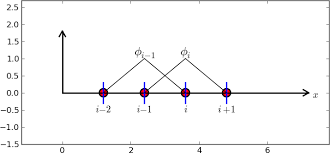
\includegraphics{FIGURES/PoissonEqn/hat_function.png}
\end{figure}
We now show that the hat functions $\phi_i$ form a basis for the space $S^h$ (Figure \ref{hatfun}).
\begin{lemma}
The set of functions $\{\phi_i \}_i^n$ is a basis for the space $S^h$.
\end{lemma}
\begin{proof}
We show first that the set $\{\phi_i \}_{1}^n$ is linearly independent.
If
$\sum_{1}^n c_i \phi_i(x) =0$ for all $x \in [a,b]$, then taking $x=x_j$, implies
$c_j=0$ for each value of $j$, and hence the functions are independent.\\
To show $S^h=\mbox{span}\{\phi_i \}$, we only need to show that
\[v(x)=v_{I}=\sum v_j\phi_j, \mbox{ all } v(x) \in S^h \]
This is proved by construction. Since $(v-v_{I})$ is linear on $[
x_{i-1},x_i]$ and $v-v_{I}=0$ at all points $x_j$, it follows that $v=v_I$ on $E_i$.
\end{proof}
We now consider the matrix $A\hat{u}=\hat{F}$ in the case where the basis functions
are chosen to be the "hat functions". In this case the elements of $A$ can be found
We have
\[\phi_i=0, \phi_i^{'}=0, \mbox{ for }  x\notin [x_{i-1},x_{i+1}) = E_{i}\bigcup E_{i+1},\]
where
\[\phi_i=\frac{x-x_{i-1}}{x_i-x_{i-1}}=\frac{1}{h_i}(x-x_{i-1}), \ \  \phi_i^{'}=\frac{1}{h_{i}}, \mbox{ on }  E_{i}.\]
and
\[\phi_i=\frac{x_{i+1}-x}{x_{i+1}-x_{i}}=\frac{1}{h_{i+1}}(x_{i+1}-x), \ \ \phi_i^{'}=\frac{-1}{h_{i+1}}, \mbox{ on }  E_{i+1}.\]
Therefore we have the elements of the matrix $A$
\[\begin{array}{ll}
A_{i,i}&=\int_{x_{i-1}}^{x_{i}}\frac{1}{h_i^2}p(x)dx +\int_{x_{i}}^{x_{i+1}}\frac{1}{h_{i+1}^2}p(x)dx \\
&+\int_{x_{i-1}}^{x_{i}}\frac{1}{h_i^2}(x-x_{i-1})^2q(x)dx +\int_{x_{i}}^{x_{i+1}}\frac{1}{h_{i+1}^2}(x_{i+1}-x)^2q(x)dx ,
\end{array}
 \]
\[\begin{array}{ll}
A_{i,i+1}&=\int_{x_{i}}^{x_{i+1}}\frac{-1}{h_{i+1}^2}p(x)dx 
+\int_{x_{i}}^{x_{i+1}}\frac{1}{h_{i+1}^2}(x_{i+1}-x)(x-x_i)q(x)dx, 
\end{array}
 \]
\[\begin{array}{ll}
A_{i,i-1}&=\int_{x_{i-1}}^{x_{i}}\frac{-1}{h_{i}^2}p(x)dx 
+\int_{x_{i}}^{x_{i+1}}\frac{1}{h_{i}^2}(x_{i}-x)(x-x_{i-1})q(x)dx, 
\end{array}
 \]
and
\[\begin{array}{ll}
F_{i}&=\int_{x_{i-1}}^{x_{i}}\frac{1}{h_{i}}(x-x_{i-1})f(x)dx 
+\int_{x_{i}}^{x_{i+1}}\frac{1}{h_{i+1}}(x_{i+1}-x)f(x)dx. 
\end{array}
 \]
\subsection{Error bounds of Finite Element methods}
\begin{lemma}
Assume $u_S$ solves $\mathbf{(W_S)}$. Then
\[a(u-u_S,w)=0, \mbox{  for all } x \in S \]
\end{lemma}

\begin{proof}
Given that
\[a(u_S,w)=(f,w), \]
and
\[a(u,w)=(f,w), \]
for all $w \in S$. Since $a$ is bilinear, taking the differences gives
\[a(u-u_S,w)=0. \]
\end{proof}

The error bounds we are interested in will be in term of the energy norm,
\[||v||_E=[a(v,v)]^{\frac{1}{2}} \]
for all $v\in D_L$.  The function satisfies the properties:
\[||\alpha v||_E=\alpha ||a||_E, \ \ \ ||v+z||_{E}\leq ||v||_E+||z||_E \]

\begin{theorem}
To show $u_{S}$ is the best fit we show that
\[||u-u_S||_E = \min_{v\in S}||u-v||_E \]
\end{theorem}
\begin{proof}
By the Cauchy -Schwarz Lemma, we have $|a(u,v)|\leq ||u||_E||v||_E$.
Let $w=u_S-v \in S$. Using the previous lemma we obtain
\[\begin{array}{ll}
||u-u_S||^2_E & = a(u-u_s,u-u_s)\\
& \leq a(u-u_s,u-u_s)+a(u-u_s,w)\\
& \leq a(u-u_s,u-u_s+w)=a(u-u_s,u-v)\\
& \leq ||u-u_s||_{E}||u-v||_E.
\end{array} \]
If $||u-u_S ||_E=0$, then the theorem holds. Otherwise
\[\min ||u-v||_E\leq ||u-u_S|| \leq \min||u-v||_E, \]
the result follows.
\end{proof}
\begin{theorem}
Error bounds
\[||u-u_S||_E \leq C h||u^{''}||_\infty\]
where C is a constant.
\end{theorem}
\begin{proof}
First from the previous theorem we have that
\[||u-u_S||_E = \min_{v\in S}||u-v||_E \leq ||u-u_I||_E\]
We look for a bound on $||u-u_I||_E$, where 
\[u_{I}(x) = \sum_j \bar{u_j} \phi_j, \ \ \ \bar{u_j}=u(x_j). \]
We assume that 
\[u_{S}(x) = \sum_j u_j \phi_j\] 
where $\mathbf{u}=\{u_j\}$ solves $A\mathbf{u}=\mathbf{F}$.
We define $e=u-u_I$. Since $u_I\in S$ implies that $u_I$ is piecewise
linear, then $u^{''}_I=0$. Therefore $e^{''}=u^{''}$.
Looking at the subinterval $[x_i,x_{i+1}]$
The Schwarz inequality yields the estimate
\[(e)^2 \leq \int_{x_i}^x 1^2 d \xi \int_{x_i}^{x}(e'(\xi))^2d \xi \]
\[ \leq (x-x_i) \int_{x_i}^{x}(e'(\xi))^2d \xi \]
\[ \leq h_i \int_{x_i}^{x_{i+1}}(e'(\xi))^2d \xi \]
and thus 
\[||e||^2_{\infty} \leq  h_i \int_{x_i}^{x_{i+1}}(e'(\xi))^2d \xi\leq h_i^2 ||e^{'}||^2_{\infty} \]
Similarly,
\[(e^{'})^2 \leq \int_{x_i}^x 1^2 d \xi \int_{x_i}^{x}(e^{''}(\xi))^2d \xi \]
\[ \leq (x-x_i) \int_{x_i}^{x}(e{''}(\xi))^2d \xi \]
\[ \leq h_i \int_{x_i}^{x_{i+1}}(e^{''}(\xi))^2d \xi \]
and thus 
\[||e^{'}||^2_{\infty} \leq  h_i \int_{x_i}^{x_{i+1}}(e^{''}(\xi))^2d \xi\leq h_i^2 ||e^{''}||^2_{\infty} \]
Finally we also have
\[
\begin{array}{ll}
a(e,e) =& \int_{x_i}^{x_{i+1}} (p(x)[e^{'}]^2 +q(x)[e(x)]^2)dx \\
& \leq ||p||_{\infty}\int_{x_i}^{x_{i+1}} [e^{'}]^2 +||q||_{\infty}\int_{x_i}^{x_{i+1}} [e(x)]^2dx \\
& \leq ||p||_{\infty}h_i^2 ||e^{''}||^2_{\infty}+||q||_{\infty}h_i^2 ||e^{'}||^2_{\infty} \\
& \leq ||p||_{\infty}h_i^2 ||e^{''}||^2_{\infty}+||q||_{\infty}h_i^4 ||e^{'}||^2_{\infty} \\
& \leq C h_i^2 ||u^{''}||^2_{\infty}
\end{array}
\]
\[||u-u_S||_E = \min_{v\in S}||u-v||_E \leq ||u-u_I||_E \leq C h ||u^{''}||_{\infty}
 \]
where $h=max\{h_{i}\}$.
\end{proof}


